\documentclass[french]{article}

\usepackage{amsmath} % for \text
\usepackage{amssymb} % for \mathbb
\usepackage{amsthm} % for proof environment
\usepackage{hyperref} % for \autoref
\usepackage{cleveref} % for \cref
\usepackage{tikz} % for tikzpicture
\usepackage{graphicx} % for \includegraphics
\usepackage{subcaption} % for subfigure
\usepackage{float} % for H in figure
\usepackage{geometry} % for \newgeometry
\usepackage{fullpage} % for fullpage
\usepackage{babel} % for french
\usepackage[T1]{fontenc} % for french
\usepackage{minted} % for code
\usepackage{xcolor} % to access the named colour LightGray


\definecolor{LightGray}{gray}{0.9}


\geometry{left = 1.8cm, right = 1.8cm}

\begin{document}

\begin{center}
    \textbf{\LARGE{Ecole Normale Supérieure de Paris-Saclay}}\\
\end{center}

\vspace{1cm}

\begin{center}
    \textbf{Rapport TER}
\end{center}

\noindent\rule{\textwidth}{0.6mm}
\bigskip
\begin{center}
    \textbf{\LARGE{TER - Voiture autonomes avec apprentissage par renforcement et lidar}}
\end{center}
\bigskip
\noindent\rule{\textwidth}{0.6mm}

\begin{center}
    \today
\end{center}

\bigskip
\begin{center}
    \textsc{Miquel Hugo}
\end{center}
\begin{center}
    \textsc{Plus Basile}
\end{center}

\begin{figure}[b]
    \centering
    \begin{minipage}[h]{0.45\textwidth}
        \raggedright
        
\includegraphics[width=0.6\textwidth]{Images/Logo-ENS-Paris-Saclay.png}
    \end{minipage}
    \begin{minipage}[h]{0.45\textwidth}
        \raggedleft
        
\includegraphics[width=0.6\textwidth]{Images/Logo-Universite-Paris-Saclay.jpg}
    \end{minipage}
\end{figure}


\newpage

\tableofcontents

\newpage

\section{Introduction}

\subsection{Contexte}

Les voitures autonomes sont un sujet de recherche très actif depuis quelques années. 
En effet, elles pourraient révolutionner le monde des transports en permettant de réduire les accidents de la route, 
de diminuer la consommation d'énergie et de réduire les embouteillages. 
Cependant, il reste encore de nombreux défis à relever pour que les voitures autonomes soient utilisées à grande échelle.
En particulier, il est nécessaire de développer des algorithmes d'apprentissage par renforcement qui permettent à une 
voiture autonome d'apprendre à conduire de manière autonome.

\subsection{Objectif et travail réalisé}
L'objectif de ce TER est de développer un algorithme d'apprentissage par renforcement qui permet à une 
voiture RC au format $1/10^{\text{ème}}$ de conduire de manière autonome sur un circuit. Dans un premier temps, nous 
avons utilisé Webots pour la simulation, gym et stable baselines pour l'apprentissage par renforcement.
Dans un second temps, nous avons transféré le réseau de neurones du simulateur à la voiture réelle.
La voiture est équipée d'un lidar qui permet de mesurer la distance entre la voiture et les murs du circuit.

\vspace{0.5cm}
\noindent
Note: Presenter Webots, la voiture réelle, la voiture sur simulateur, le lidar, le circuit etc...


\subsection{L'apprentissage par renforcement}
L'apprentissage par renforcement est une méthode d'apprentissage automatique qui permet à un agent 
d'apprendre à prendre des décisions en interagissant avec un environnement. 

\begin{figure}[H]
    \centering
    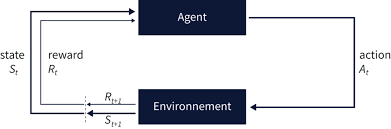
\includegraphics[width=0.6\textwidth]{Images/RL.png}
    \caption{Schéma de l'apprentissage par renforcement}
\end{figure}

L'agent prend des actions dans l'environnement et reçoit une récompense en fonction de l'action qu'il a prise. 
L'objectif de l'agent est de maximiser la somme des récompenses qu'il reçoit au cours des itérations.

\vspace{0.5cm}
Lors de chaque étape, l'agent reçoit une observation de l'environnement dans lequel il évolue. Sur la base 
de cette observation, l'agent prend une décision parmi un ensemble d'actions possible appelé espace des actions. 
Cet espace peut dépendre de l'état dans lequel se trouve l'agent.

\vspace{0.5cm}
Un exemple simple est celui d'un jeu d'échecs dans lequel l'observation correspond à la position de chacune des 
pièces sur l'échiquier et l'espace des actions est l'ensemble des déplacements possibles des pièces. 
Naturellement, on souhaite que l'agent réalise la meilleure action possible suivant l'observation reçue. 
Pour atteindre ce but, l'agent applique une politique d'action (notée $\pi$) qu'il utilise pour sa prise de décision.
À chaque récompense obtenue, cette politique est mise à jour. On espère ainsi atteindre une politique optimale.

\vspace{0.5cm}
Pour entraîner un agent, plusieurs types de méthodes peuvent être utilisées. Ces méthodes estiment la somme des 
récompenses futures que l'agent devrait obtenir. Ces récompenses sont pondérées pour favoriser les récompenses 
à court terme. La politique obtenue est souvent modélisée par un réseau de neurones, dont l'actualisation modifie 
les poids du réseau.

\vspace{0.5cm}
\noindent
Les méthodes d'apprentissage par renforcement peuvent être classées en trois catégories principales :
\begin{itemize}
\item \textbf{Méthodes basées sur la valeur (value-based)} : Ces méthodes se concentrent sur l'estimation de la récompense cumulative optimale que l'agent peut obtenir. Elles cherchent à obtenir une récompense cumulative maximale.
\item \textbf{Méthodes basées sur la politique (policy-based)} : Ces méthodes se concentrent sur l'optimisation de la politique de l'agent. Les valeurs de récompense peuvent ne pas être calculées directement.
\item \textbf{Méthodes acteur-critique (actor-critic)} : Ces méthodes utilisent deux réseaux de neurones. Le premier réseau choisit l'action à effectuer, tandis que le second réseau évalue cette action en la comparant à l'action prévue.
\end{itemize}


\section{Simulation}

\subsection{Le simulateur Webots}
Le logiciel utilisé pour la simulation est Webots R2023b. Webots est un logiciel de simulation de robotique développé 
par Cyberbotics. Il permet de simuler des robots dans un environnement 3D que l'on peut personnaliser. Dans notre cas,
nous avons utilisé Webots pour simuler une voiture RC sur un circuit. Nous avons utilisé le langage de programmation
Python pour contrôler la voiture dans le simulateur.

\begin{figure}[H]
    \centering
    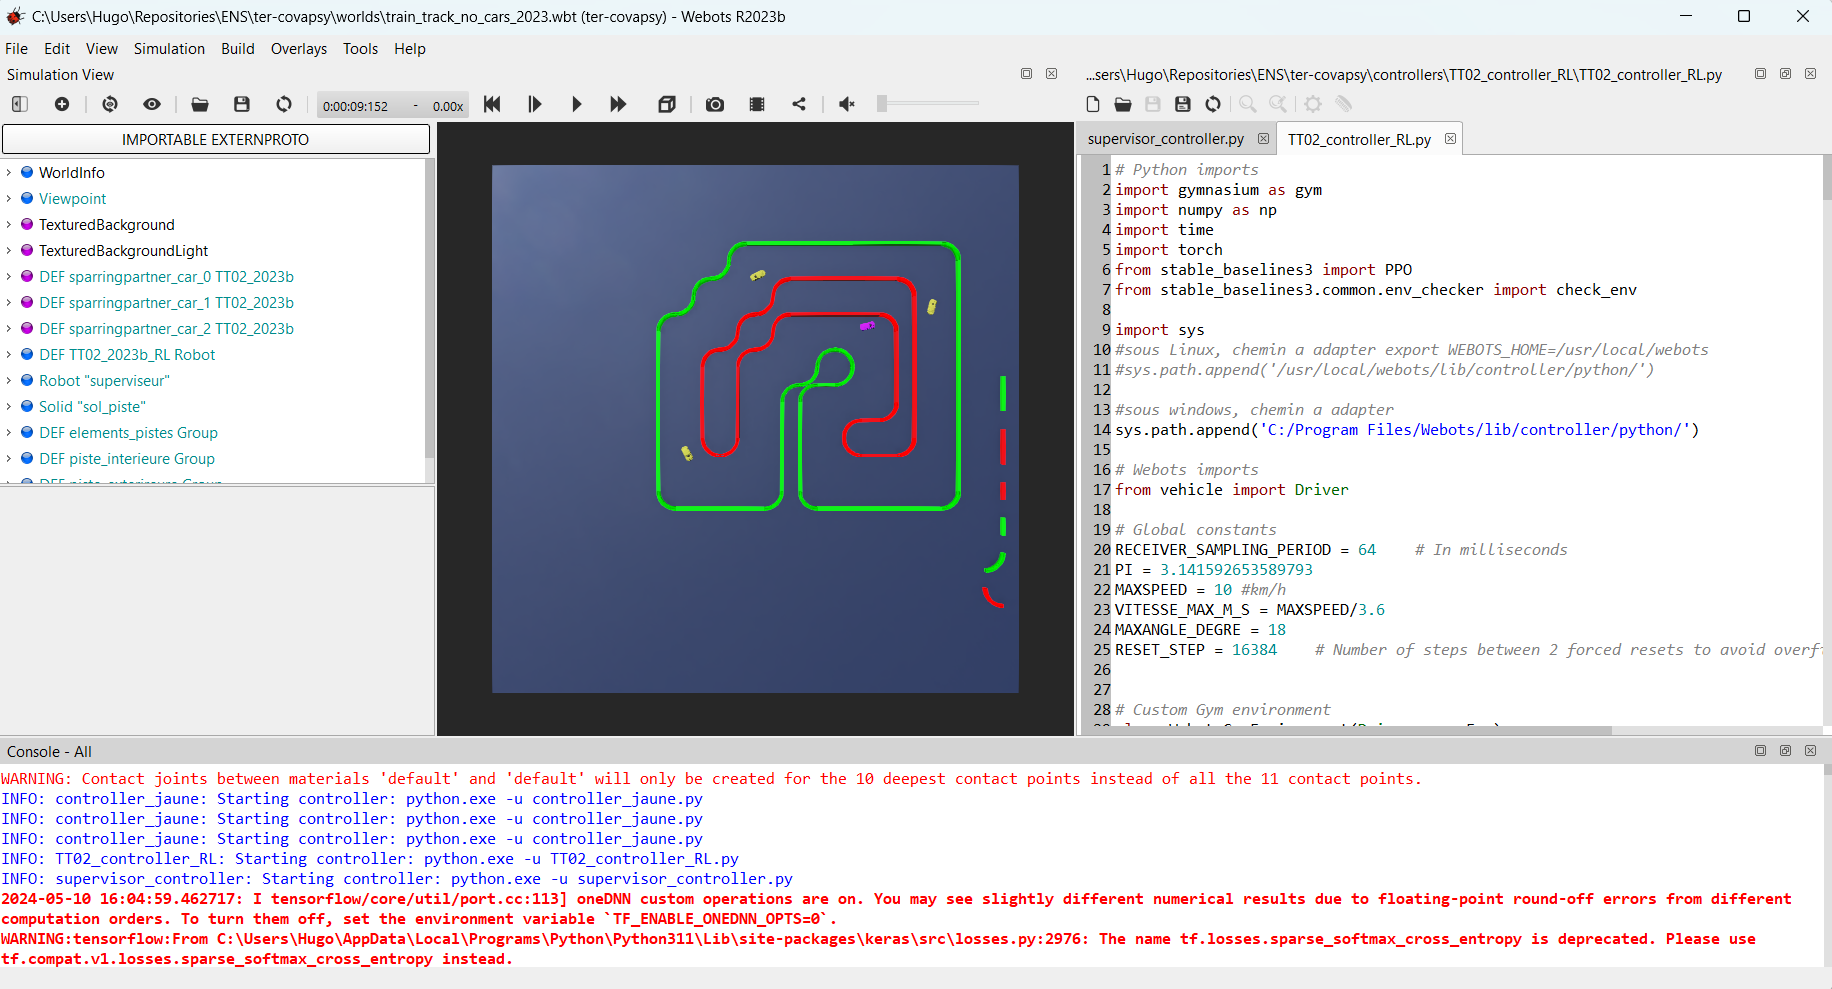
\includegraphics[width=0.9\textwidth]{Images/Webots.png}
    \caption{Capture d'écran de Webots}
\end{figure}

\noindent
Note: Présenter le circuit, la voiture, le lidar, le code Python etc...

\subsection{Le circuit}
Le circuit dans l'environment de Webots a pour but de simuler un circuit réel sur lequel la voiture autonome doit
apprendre à conduire. Les murs du circuit sont composés de blocs de couleur différentes pour les bordures extérieur et 
intérieur du circuit. Ces murs ont une auteur d'une dizaine de centimètres qui permettent au lidar de mesurer la distance
entre la voiture et les murs.

\begin{figure}[H]
    \centering
    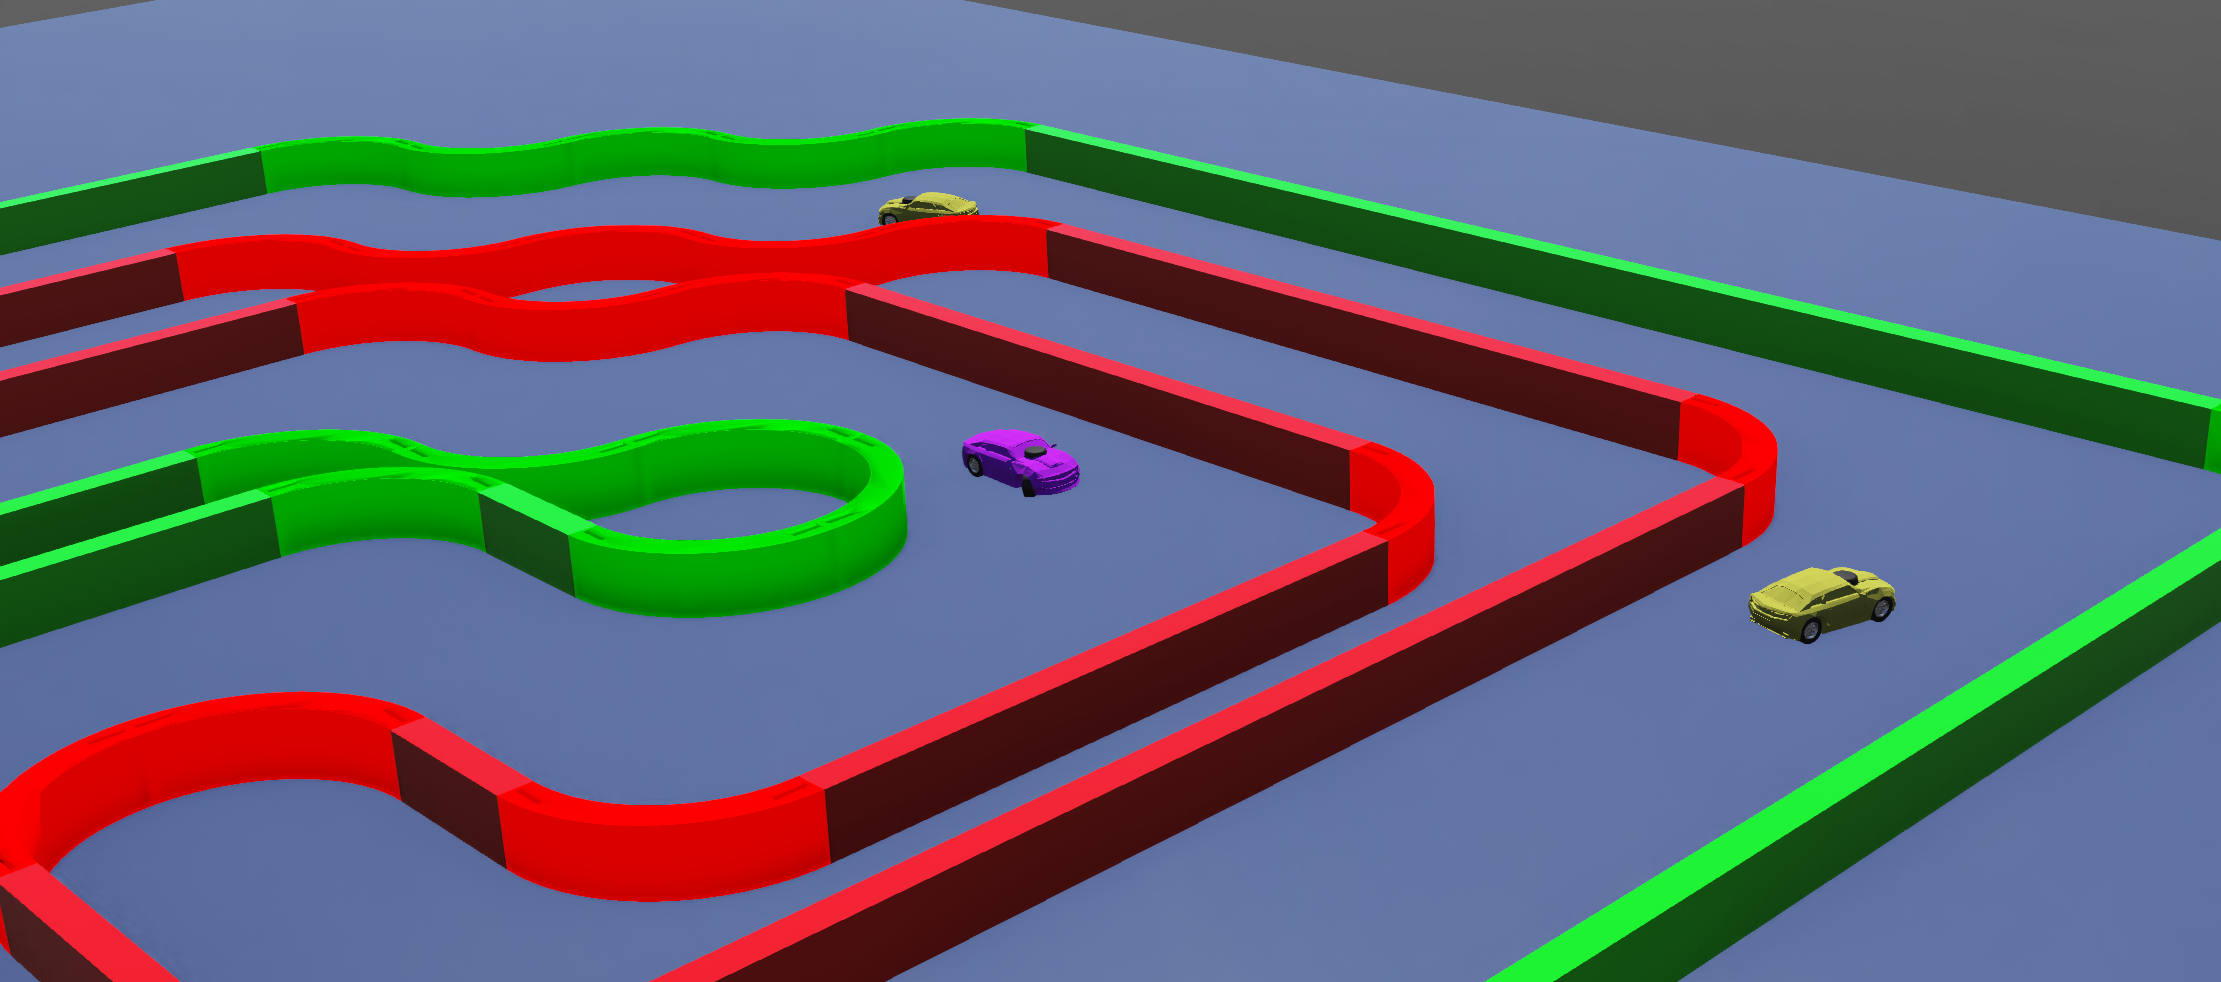
\includegraphics[width=0.9\textwidth]{Images/Circuit.png}
    \caption{Capture d'écran du circuit}
\end{figure}

\subsection{La voiture}
La voiture utilisée dans le simulateur est une voiture RC au format $1/10^{\text{ème}}$. Elle a pour objectif de
reproduire le plus fidèlement possible une voiture réelle. La voiture est équipée d'un lidar qui permet de mesurer la
distance entre la voiture et les murs du circuit.

\begin{figure}[H]
    \centering
    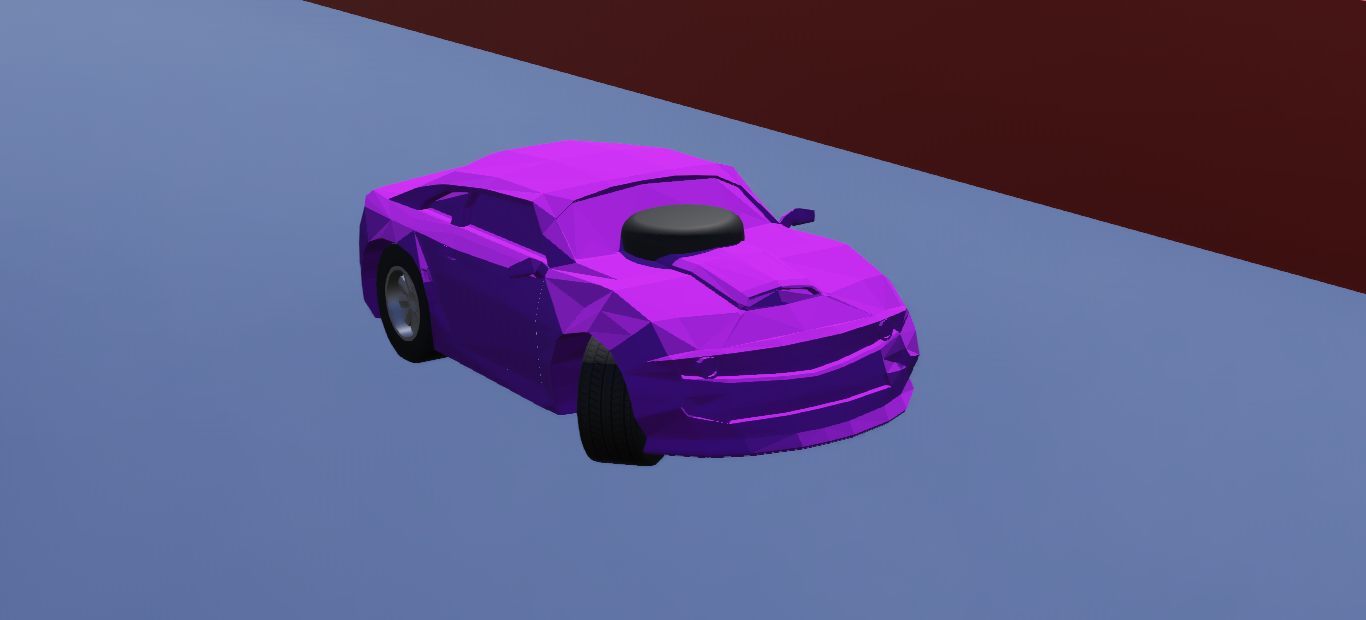
\includegraphics[width=0.9\textwidth]{Images/Voiture.png}
    \caption{Capture d'écran de la voiture}
\end{figure}

\subsection{Le lidar}


\section{Simulation to real world}
L'objectif du SimToReal est de transférer un réseau de neurones entraîné sur un simulateur à une voiture réelle. 
Une fois le réseau de neurones entraîné, il est transféré à la voiture réelle pour qu'elle puisse conduire de manière 
autonome sur un circuit réel. Un des principaux défis du SimToReal est de reproduire le plus fidèlement possible les 
conditions du monde réel dans le simulateur.

\vspace{0.5cm}
La phase d'entraînement sur simulateur a plusieurs avantages. Tout d'abord, elle permet de réduire le temps et le coût
de l'entraînement. En effet, il est possible de simuler des milliers d'épisodes en quelques heures 
alors qu'il faudrait plusieurs jours pour réaliser le même nombre d'épisodes sur une voiture réelle. De plus,
la simulation permet de tester des scénarios dangereux pour la voiture réelle sans risquer de l'endommager.
Sur la voiture réelle, il faut aussi la replacer à la main après chaque crash dans un mur. Il est donc plus
efficace de réaliser l'entraînement sur simulateur.

\section{Introduction du bruit pour améliorer la simulation}
Pour que la simulation soit la plus proche possible de la réalité, il est crucial d'introduire des éléments de bruit. 
Ces bruits peuvent affecter les mesures et les actions de la voiture, et ainsi permettre au réseau de neurones de 
mieux généraliser lors du passage au monde réel.


\subsection{Bruit sur les mesures}
Dans un environnement réel, les capteurs ne fournissent pas des mesures parfaites. Les mesures du Lidar peuvent 
toujours être affectées par de petites interférences ou des variations mineures. Pour simuler ces conditions, 
on peut ajouter un léger bruit gaussien aux mesures du Lidar. Cela permet au réseau de neurones de s'adapter 
à des données moins parfaites, similaires à celles qu'il rencontrera dans le monde réel.


\subsection{Bruit sur les actions}
Les actions de la voiture, telles que l'angle de direction ou la vitesse, peuvent également être sujettes à des 
variations imprévues. Par exemple, un servomoteur peut ne pas toujours répondre de manière identique à une même 
commande en raison de l'usure ou des variations de tension. Pour prendre en compte ces imperfections, on peut 
ajouter du bruit aux actions commandées par le réseau de neurones. Cela aide à rendre l'agent plus robuste face 
aux variations qu'il pourrait rencontrer sur une voiture réelle.



\section{Application à la voiture autonome}
Pour appliquer l'apprentissage par renforcement à une voiture autonome, il est essentiel de définir correctement 
l'espace d'observation et l'espace d'action en tenant compte des contraintes du monde réel.

\subsection{Espace d'observation}
L'espace d'observation doit inclure toutes les informations pertinentes que la voiture peut obtenir de son environnement.
Dans notre cas, nous utilisons le Lidar pour mesurer les distances aux obstacles. Si un système de contrôle de 
la vitesse est en place, la vitesse actuelle de la voiture pourrait également faire partie de l'espace d'observation.

\subsection{Espace d'action}
L'espace d'action est limité aux commandes que l'agent peut envoyer à la voiture. Cela inclut l'incrémentation de 
l'angle de direction via le servomoteur et l'incrémentation de la vitesse via le moteur.


\section{Entraînement du réseau de neurones}
\subsection{Algorithme d'apprentissage}
\subsubsection*{Circuit d'entraînement}
La piste d'entraînement utilisée est conçue pour offrir une variété de situations afin que la voiture puisse 
apprendre à gérer différentes circonstances qu'elle pourrait rencontrer en course. Le circuit est composé de virages 
à gauche et à droite, de longues lignes droites, de virages en épingle et d'une section en diagonale. 
La piste retenue est la suivante:

\begin{figure}[H]
\centering
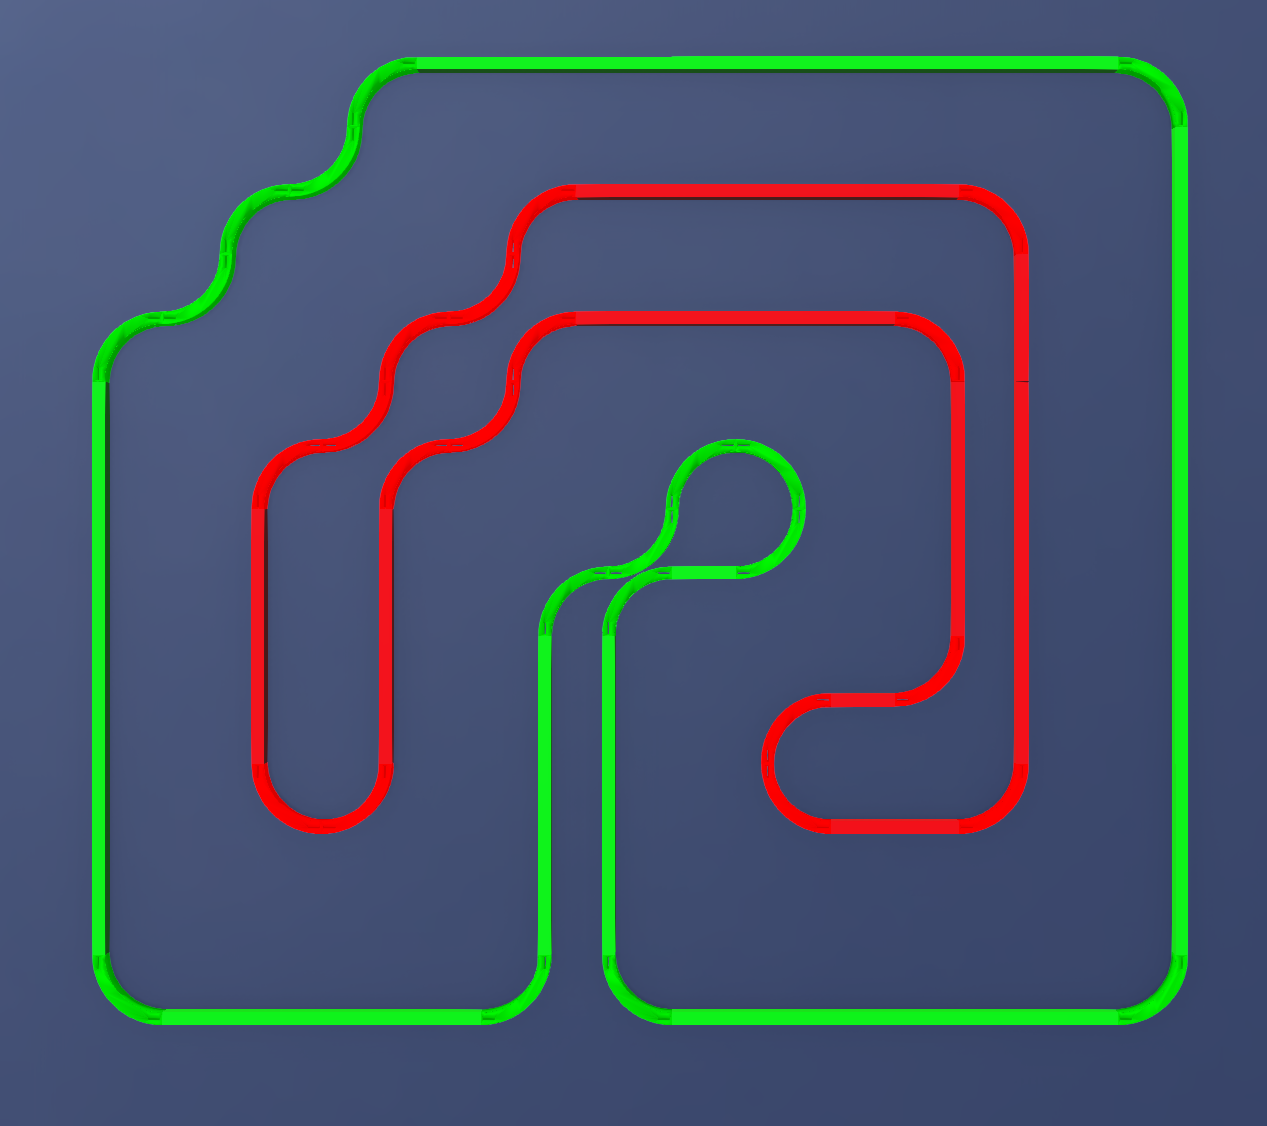
\includegraphics[width=0.8\textwidth]{Images/Piste Entrainement.png}
\caption{Piste d'entraînement pour l'apprentissage par renforcement}
\end{figure}

Sur ce circuit, nous avons ajouté trois autres voitures qui roulent à vitesse modérée pour simuler des situations 
de dépassement. Ces voitures suivent un algorithme de conduite simple qui consiste à rester à distance des murs.

\vspace{0.5cm}
Pour cet environnement, nous avons également intégré un robot "Superviseur" qui repositionne les voitures à des 
positions aléatoires lorsque nous souhaitons recommencer un épisode. Ce "Superviseur" choisit aléatoirement 
une position et une direction sur le circuit pour replacer les voitures, assurant ainsi une situation initiale 
nouvelle à chaque début d'épisode. La communication avec le "Superviseur" se fait via un système émetteur-récepteur 
intégré dans Webots.


\subsubsection*{Environment Gym}
La bibliothèque Gym est une bibliothèque implémentée en Python qui permet de gérer la partie apprentissage par 
renforcement d'un réseau de neurones. Dans le cas de notre projet, Gym ne propose pas d'environnement adapté. 
Il a donc été nécessaire de créer un tout nouvel environnement. Gym exige qu'un environnement contienne les fonctions 
suivantes:
\begin{itemize}
    \item \textbf{get\_observation()} : fonction renvoyant les observations de l'environnement
    \item \textbf{get\_reward()} : fonction donnant la récompense selon l'action effectuée par l'agent
    \item \textbf{reset()} : fonction donnant la démarche pour repartir au début d'un épisode
    \item \textbf{step()} : fonction faisant évoluer l'environnement
\end{itemize}

\vspace{0.5cm}
Toutes ces fonctions sont rassemblées dans une classe que nous avons nommée \texttt{WebotsGymEnvironment}. Dans cette classe, nous avons rajouté quatre fonctions propres à la voiture :
\begin{itemize}
\item \textbf{get\_lidar\_mm()} : Fonction qui renvoie un tableau de Lidar dans le bon format avec des valeurs cohérentes en mm.
\item \textbf{set\_vitesse\_m\_s()} : Fonction qui prend en argument une vitesse en m/s et qui la convertit en km/h avant de l'envoyer à la voiture.
\item \textbf{set\_direction\_degre()} : Fonction qui prend un angle en degré et le convertit en radian avant de l'envoyer à la voiture.
\end{itemize}
\noindent
Nous allons détailler par la suite chacune des fonctions.

\subsubsection*{get\_observation()}
Dans la fonction \texttt{get\_observation()}, on appelle la fonction \texttt{get\_lidar\_mm()} pour récupérer 
les observations du Lidar. Ce tableau sera le tableau donné en entrée du réseau pour les observations du Lidar 
à "l'instant présent". Pour ce qui est du tableau à "l'instant précédent", on stocke à chaque appel de la 
fonction le tableau d'observation dans une variable interne de la classe. Si la fonction est appelée depuis 
la fonction \texttt{reset()}, on donne le même tableau pour les deux parties de l'espace d'observation concernant 
le Lidar puisque la voiture a été repositionnée. Pour la vitesse et la direction, Webots nous permet de mesurer 
la vitesse et la direction de la voiture dans le simulateur. Ce sont ces données que l'on donne au réseau de neurones. 
De même dans le cas où l'observation est demandée par la fonction \texttt{reset()}, on indique que ces deux grandeurs 
sont nulles. Il est à noter que les valeurs données à l'espace d'observation sont normalisées.

\subsubsection*{get\_reward()}
Dans la fonction \texttt{get\_reward()}, on donne la récompense associée à l'état dans lequel se trouve la voiture. 
On distingue deux états possibles pour la voiture. Le premier état est celui d'une situation de collision. 
On regarde la plus petite valeur du tableau de Lidar actuel et si celui-ci est inférieur à 120 mm, on considère 
qu'il y a collision. Dans le cas de la collision, on donne un malus de -400 moins la vitesse de la voiture. 
Le deuxième état regroupe toutes les situations autres que celle de collision. On donne comme récompense ici 
une valeur dépendant de la vitesse actuelle de la voiture ainsi que la distance minimale donnée par le tableau de Lidar. 
Les fonctions de récompenses seront détaillées plus tard. On indique aussi ici si l'on a terminé l'épisode via la 
variable \texttt{done}.

\subsubsection*{reset()}
Dans la fonction \texttt{reset()}, on indique la démarche à suivre lorsque l'on veut retourner au début d'un épisode. 
Le reset se fait dans le cas d'un crash de la voiture ou si le nombre d'actions autorisées par épisode est atteint. 
Au moment du reset, on donne des consignes de vitesse et d'angle nuls et on envoie une indication de reset au robot 
"Superviseur". À la fin de la routine de réinitialisation, on renvoie une observation.

\subsubsection*{step()}
Dans la fonction \texttt{step()}, on indique que l'on fait un pas dans le processus d'apprentissage. Dans cette 
fonction, on fait avancer la voiture avec les actions récupérées depuis le réseau de neurones. Ensuite, on récupère 
une observation depuis le Lidar et on fait faire un pas au processus d'apprentissage. On calcule la récompense 
avant de retourner toutes les informations obtenues.

\subsection{Réseau de neurones avec Stable-Baselines3}
La librairie Stable-Baselines3 permet de créer un réseau de neurones géré par l'algorithmes d'apprentissage 
par renforcement PPO (Proximal Policy Optimization). Stable-Baselines3 propose un large choix de paramètres pour 
l'apprentissage. Voici un descriptif des paramètres utilisés ainsi que leurs valeurs définies dans notre programme:
\begin{itemize}
    \item \textbf{policy} : Type de politique utilisée. Dans notre cas, nous utilisons 'MultiInputPolicy' 
    pour gérer les multiples entrées.
    \item \textbf{env} : Environnement d'apprentissage Gym.
    \item \textbf{learning\_rate} : Taux d'apprentissage fixé à $5 \cdot 10^{-4}$.
    \item \textbf{n\_steps} : Nombre d'actions autorisées par épisode (2048).
    \item \textbf{batch\_size} : Taille du lot de données pour chaque mise à jour (64).
    \item \textbf{n\_epochs} : Nombre d'époques d'entraînement par itération de \texttt{n\_steps} (10). 
    \item \textbf{gamma} : Facteur de discount pour la récompense future (0.99).
    \item \textbf{gae\_lambda} : Facteur pour le calcul de l'estimateur de l'avantage généralisé (0.95).
    \item \textbf{clip\_range} : Valeur de clipping pour PPO (0.2).
    \item \textbf{vf\_coef} : Coefficient de la fonction de perte de la valeur (1).
    \item \textbf{ent\_coef} : Coefficient d'entropie pour la fonction de perte (0.01).
    \item \textbf{device} : Composant sur lequel faire tourner l'algorithme (dans notre cas, 'cuda:0' pour l'utilisation du GPU).
    \item \textbf{tensorboard\_log} : Emplacement pour enregistrer les données de Tensorboard ('./PPO\_Tensorboard').
\end{itemize}
Voici un extrait de notre code de définition de modèle :
\begin{minted}[
    frame=lines,
    framesep=2mm,
    baselinestretch=1.2,
    bgcolor=LightGray,
    fontsize=\footnotesize,
    linenos
]
{python}
# Définition du modèle
model = PPO(
    policy="MultiInputPolicy",
    env=env,
    learning_rate=5e-4,
    verbose=1,
    device='cuda:0',
    tensorboard_log='./PPO_Tensorboard',
    # Paramètres additionnels
    n_steps=2048,
    batch_size=64,
    n_epochs=10,
    gamma=0.99,
    gae_lambda=0.95,
    clip_range=0.2,
    vf_coef=1,
    ent_coef=0.01
)
\end{minted}

Nous pouvons ensuite entraîner le modèle avec la fonction \texttt{model.learn()}. Cette fonction prend en argument
le nombre d'itérations d'entraînement. Une fois l'entraînement terminé, nous pouvons sauvegarder le modèle avec
la fonction \texttt{model.save()}.Nous pouvons dans un second temps charger le modèle avec la fonction 
\texttt{model.load()} ce qui nous permet, par exemple de reentrainer le modèle avec de nouveau paramètres ou avec 
une nouvelle fonction de récompense. Nous pouvons également visualiser les données d'entraînement avec Tensorboard
en exécutant la commande \texttt{tensorboard --logdir ./PPO\_Tensorboard}.


\subsection{Fonction de récompense}
La fonction de récompense est un élément crucial de l'apprentissage par renforcement. Elle permet de guider
l'agent vers les actions qui maximisent la récompense. C'est un élément délicat à définir car une mauvaise
fonction de récompense peut entraîner des comportements indésirables de l'agent. En effet si l'on ne prend pas 
assez en compte le crash de la voiture, l'agent pourrait apprendre à foncer dans les murs pour maximiser la vitesse.
Si l'on ne prend pas en compte la vitesse, l'agent pourrait apprendre à rester immobile pour éviter les collisions et
rester éloigné des murs. Il est donc important de trouver un équilibre entre ces aspects. 

\vspace{0.5cm}
Dans notre cas, nous avons défini une fonction de récompense qui prend en compte la vitesse de la voiture et la distance
minimale donnée par le Lidar. La récompense est définie comme suit:

\begin{equation}
    \text{reward} = \begin{cases}
        -400 - 10 * \text{vitesse} & \text{si collision} \\
        18 * (\text{mini} - 0.018) + 2 * \text{vitesse} & \text{sinon}
    \end{cases}
\end{equation}

Où $\text{mini}$ est la distance minimale donnée par le Lidar et $\text{vitesse}$ est la vitesse de la voiture.
La récompense est négative en cas de collision et dépend de la vitesse de la voiture. Cela permet de fortement pénaliser
les collisions à haute vitesse. Dans le cas où il n'y a pas de collision, la récompense dépend de la distance minimale
donnée par le Lidar et de la vitesse de la voiture. Cela permet de favoriser les actions qui permettent à la voiture
de rouler vite tout en restant loin des murs pour éviter les collisions.

\vspace{0.5cm}
Nous avons également essayé de prendre en compte le temps de passage au tour. Pour cela, nous avons adapté le 
superviseur afin de détecter les passages sur la ligne d'arrivée et de notifier la fonction de récompense pour 
donner une récompense positive lors d'un passage sur la ligne d'arrivée. Plus le temps au tour est court, plus 
la récompense est élevée. Cela permet de former la voiture à vraiment aller vite et à réaliser un temps au tour 
le plus rapide possible. Cette approche encourage l'agent à optimiser non seulement la vitesse et la sécurité, 
mais aussi l'efficacité globale de ses déplacements sur le circuit.


\subsection{Mise en place de la simulation}
Après avoir défini l'environnement Gym, le réseau de neurones et la fonction de récompense, nous pouvons lancer
l'entraînement de la voiture autonome.

\subsubsection*{Entraînement}
La première étape consiste à déclarer l'environnement Gym et à vérifier que celui-ci est correctement défini avec 
la fonction \texttt{check\_env()}:

\begin{minted}[
    frame=lines,
    framesep=2mm,
    baselinestretch=1.2,
    bgcolor=LightGray,
    fontsize=\footnotesize,
    linenos
]{python}
env = WebotsGymEnvironment()
check_env(env)
\end{minted}

Après cela, nous pouvons définir le modèle et lancer l'entraînement avec la fonction \texttt{model.learn()}. Nous 
donnons en argument \texttt{total\_timesteps} qui correspond au nombre total d'itérations d'entraînement. Nous 
pouvons ensuite sauvegarder le modèle avec la fonction \texttt{model.save()} qui prend en argument le nom du fichier
de sauvegarde.

\section*{Passage à la voiture réelle}
Une fois le réseau de neurones entraîné sur le simulateur, nous pouvons le transférer à la voiture réelle. C'est 
la dernière étape du projet. Cette transition du monde virtuel au monde réel nécessite une adaptation des algorithmes 
et des fonctionnalités pour s'adapter aux contraintes et aux spécificités de la réalité.

\subsubsection*{Adaptation des commandes}
Pour garantir une interprétation adéquate des commandes générées par le réseau de neurones sur la voiture réelle,
nous avons développé deux fonctions équivalentes à celles utilisées dans le simulateur : \texttt{set\_vitesse\_m\_s()} 
et \texttt{set\_direction\_degre()}. Toutefois, cette fois-ci, les commandes sont transmises en m/s et en degrés de 
direction au lieu d'être directement appliquées. De plus, pour le Lidar, nous avons pris soin de traiter les données 
afin d'éviter les valeurs nulles dans les parties "utiles" du Lidar.


\subsubsection*{Chargement du réseau de neurones}
Le chargement du réseau de neurones a été effectué en utilisant la fonction \texttt{load()} de la bibliothèque 
Stable-Baselines3. Une fois chargé, le réseau peut être utilisé via la fonction \texttt{predict()}, prenant en 
entrée les observations et renvoyant les actions prédites. Toutefois, contrairement à la simulation, l'accès direct 
à la vitesse et à la direction n'est pas possible en raison de l'absence de système d'asservissement. Seules les 
consignes de vitesse et d'angle de l'instant précédent sont fournies en tant qu'observations.

\subsubsection*{Lidar}
Pour exploiter le Lidar, nous avons mis en place une classe \texttt{Lidar\_TT02()} pour initialiser, démarrer 
et acquérir les valeurs du Lidar. Deux threads ont été lancés : \texttt{thread\_scan\_lidar} pour une acquisition 
continue des données Lidar, et \texttt{thread\_conduite\_autonome} pour la gestion du pilotage de la voiture. 
Dans la fonction \texttt{conduite\_autonome()}, les données Lidar sont traitées pour prendre des décisions, 
telles que reculer en cas de détection d'obstacle.

\subsection{Résultats}

Dans un premier temps nous avons testé la voiture avec un des réseau de neurones qui nous semblait le plus performant.
Dans un premier temps nous faisons tourner la voiture seul sur un circuit sans obstacles, c'est la phase de 
qualification. La voiture est évaluée sur le temps qu'elle met pour faire deux tours du circuit. Notre voiture a
réalisé un temps de 30,22 secondes à la première manche de la qualification. La deuxième phase de la qualification
consiste à faire tourner la voiture sur un circuit avec des obstacles. Notre voiture n'a pas réussi à terminer le
circuit et a été arrêtée par un obstacle, le temps retenue a été de 90 secondes. La voiture a donc réalisé un temps
total de 120,22 secondes la plaçant en $11^{eme}$ position de la qualification.

\begin{figure}[H]
    \centering
    \includegraphics[width=0.8\textwidth]{Images/2_EssaisLibresEtQualifications_48.JPG}
    \caption{Piste de qualification avec obstacles}
\end{figure}

Suite à cela, toutes les voitures sont mises en piste pour une course de 5 tours. Notre voiture a terminé en première 
position de la manche 2 de la course.

\begin{figure}[H]
    \centering
    \includegraphics[width=0.8\textwidth]{Images/4_Courses_29.JPG}
    \caption{Piste de course}
\end{figure}

Une observation faites lors de la course est que la voiture se déplace en "zigzag" sur les lignes droites. Ce 
comportement était déjà present sur le simulateur mais moins prononcé. Ce problème est probablement dû à un manque
de précision dans le modèle de la simulation sur le simulateur. Un des paramètres de la voiture dans le simulateur
est le couple maximale du servomoteur de la direction. Ce paramètre est fixé dans la simulation Webots à une valeur
beaucoup trop élevée par rapport à la réalité. Cependant, baissé ce paramètre dans la simulation Webots a pour
conséquence de complètement casser la simulation, la voiture n'avance plus sur le simulateur. C'est un problème 
à résoudre pour améliorer la simulation.

\vspace{0.5cm}
Un autre point qui pourrait améliorer les déplacements en "zigzag" de la voiture est d'ajouter un terme pénalisant 
le fait de changer de direction dans la fonction de récompense. Cela permettrait potentiellement d'encourager la 
voiture à rester dans la même direction lorsqu'elle est sur une ligne droite. C'est une piste d'amélioration pour 
la suite du projet.


    



\section{Conclusion}





Note:
Il faut ajouter la partie ou on améliore la simulation Webots avec les obstacles, Basile l'a fait.



\end{document}